\section{Trabalhos relacionados}

Esta seção apresenta projetos relacionados a este, bem como uma comparação entre os mesmos.

\subsection{PeLeP}

O projeto PeLeP, apresentado por Levis et al\cite{pelep}, busca integrar a utilização de perfis com aperfeiçoamento automático com ambientes de educação ubíqua.

Os ambientes de \emph{computação ubíqua} são parte de um cenário na qual serviços e informações estão disponíveis a qualquer momento, em qualquer lugar\cite{weiser91}. Esta visão vem sendo potencializada pela diminuição do custo e aumento da capacidade de memória e processamento dos dispositivos computacionais, bem como pela cada vez maior disponibilidade de recursos de localização e conectividade. A computação ubíqua enfatiza também a ``tecnologia calma'', onde a sobrecarga de informação é substituída pela disponibilização de recursos de forma inteligente, tomando a atenção do usuário apenas nos momentos em que é mais relevante.\cite{weiser96}

Levis et al compreendem \emph{educação ubíqua} como sendo processos educacionais que ocorrem em qualquer lugar, a qualquer tempo e com qualquer dispositivo, de forma contínua, contextualizada e integrada ao cotidiano do aprendiz. Desta forma, o conhecimento presente no dia-a-dia das mais diferentes formas e em diferentes locais podem ser relacionados com processos educacionais direcionados aos aprendizes.

O PeLeP, cujo modelo é ilustrado na Figura~\ref{fig:pelep1}, é um modelo dedicado ao gerenciamento de perfis de aprendizes em um ambiente ubíquo de ensino e aprendizagem. O modelo administra os perfis automaticamente, inferindo informações através do histórico do aprendiz. As alterações realizadas no perfil refletem o comportamento do aprendiz no ambiente ubíquo, levando em consideração o seu modelo de mobilidade e de contexto.

\begin{figure}
  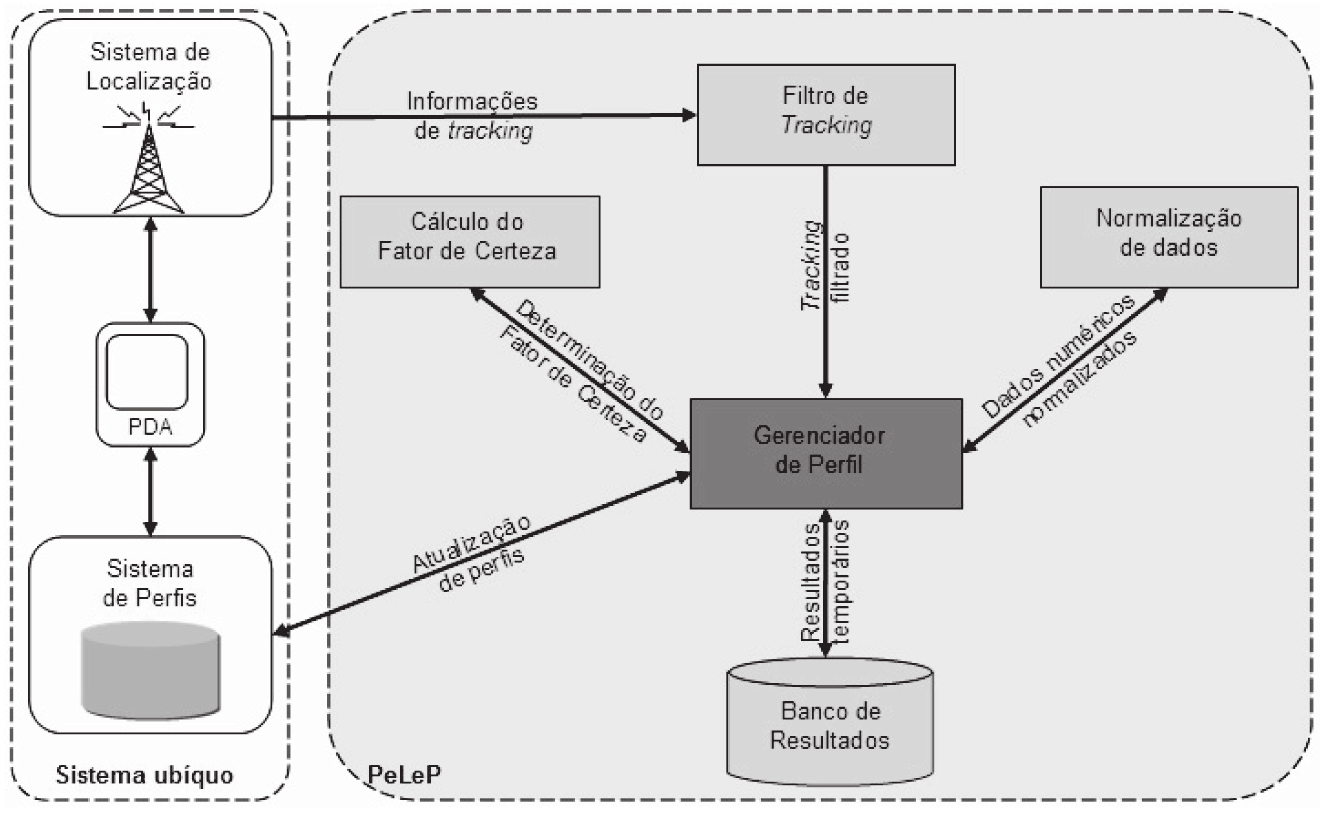
\includegraphics[width=0.5\textwidth]{imagens/pelep1.png}
  \caption{Arquitetura do PeLeP\cite{pelep}}
  \label{fig:pelep1}
\end{figure}


\subsection{Chellouche et al}

O artigo de Chellouche et al\cite{chellouche10} discute as dificuldades atuais no desenvolvimento de aplicativos para dispositivos móveis, uma vez que os mesmos possuem uma grande variedade de resolução, memória, poder computacional, etc. Além disso, a qualidade da conexão de um usuário pode variar grandemente, e isto também deve ser levado em consideração no desenvolvimento.

O conjunto de informações que caracteriza um usuário é chamada de \emph{perfil de usuário}. Com a intenção de compartilhar o contexto do usuário entre serviços e minimizar as mudanças no desenvolvimento de aplicações sensíveis a contexto, os autores propõem como solução um \emph{middleware} que gerencia o perfil de um usuário dinamicamente e supre às aplicações todas as informações que elas podem precisar durante o período de adaptação.

O perfil do usuário é constituído por seu contexto, onde a definição de contexto utilizada é aquela dada por Dey\cite{dey2001}, na qual contexto refere-se a qualquer informação que pode ser utilizada para caracterizar a situação de uma entidade. Assim, o perfil de usuário é dividido em cinco componentes:

\begin{description}
  \item[Perfil geral]: refere-se às informações básicas, como nome, endereço, telefone, idade, sexo, etc. Inclui também possíveis deficiências pessoas do usuário.
  \item[Perfil do dispositivo]: informações a respeito dos dispositivos do usuário, tais como marca, capacidade, sistema operacional, etc.
  \item[Perfil de rede]: descreve as redes às quais o usuário pode se conectar, com suas características.
  \item[Perfil dos serviços]: registra as informações a respeito de serviços, como nome, versão, porta e conteúdo.
  \item[Perfil de contexto]: contém informações a respeito do ambiente do usuário, como hora, data e localização, aplicações em execução, banda disponível, etc. É considerada a parte dinâmica do perfil, composta por dados voláteis.
\end{description}

O \emph{middleware} é apresentado segundo ilustrado na Figura~\ref{fig:chellouche1}. O \emph{middleware} é composto dos seguintes módulos:

\begin{figure}
  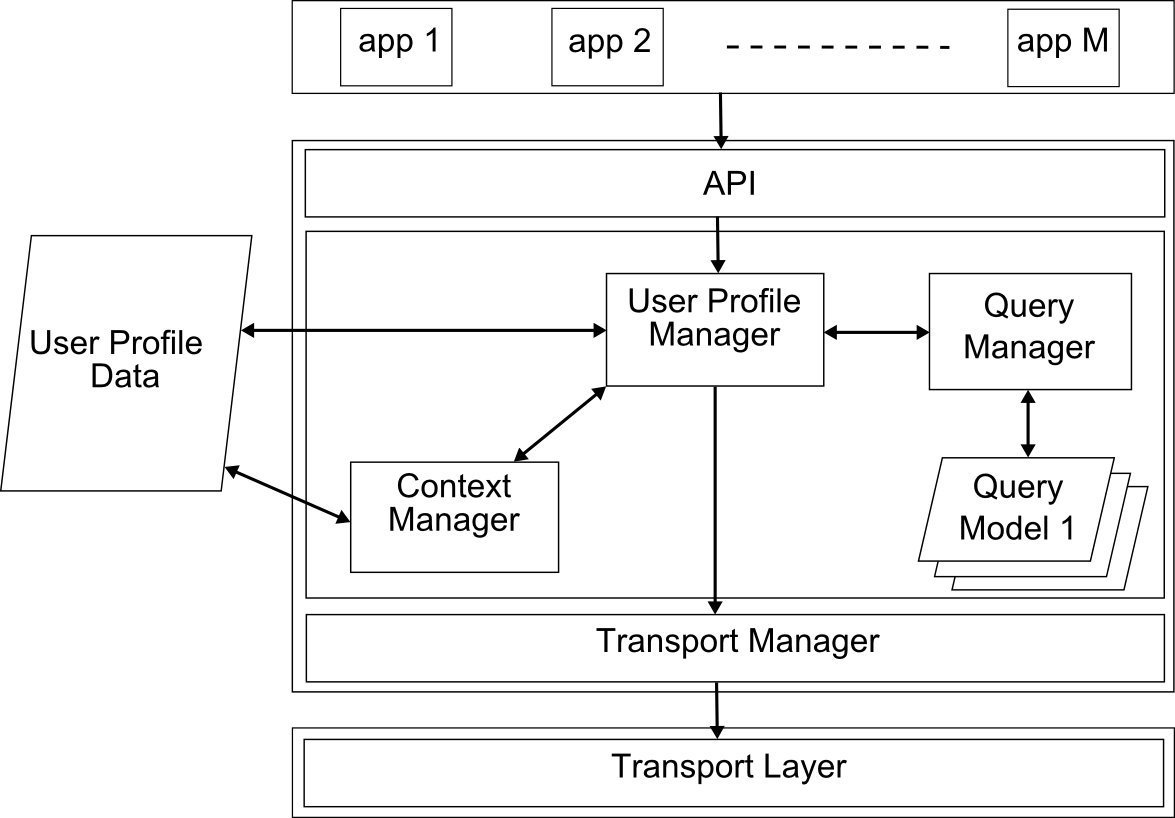
\includegraphics[width=0.5\textwidth]{imagens/chellouche1.png}
  \caption{Arquitetura do \emph{middleware} de Chellouche et al\cite{chellouche10}}
  \label{fig:chellouche1}
\end{figure}

\begin{description}
  \item[User profile manager]: módulo central da arquitetura, que interage com todos os outros módulos com o objetivo de construir o perfil correto.
  \item[Context manager]: monitora o ambiente, coletando informações com o objetivo de atualizar a parte dinâmica do perfil.
  \item[Query manager]: módulo responsável por validar e salvar um modelo de consulta para cada aplicação. É construída quando a aplicação é instalada e utilizada quando a aplicação solicita informações.
  \item[Transport manager]: faz a comunicação do perfil de usuário para a aplicação.
  \item[API]: constitui o ponto de interface entre as aplicações e o middleware.
\end{description}

O perfil é construído de acordo com a Figura~\ref{fig:chellouche2}. A aplicação solicita ao gerenciador de perfis, através da API, que por sua vez repassa a solicitação ao gerenciador de consultas. Simultâneo a isto, o gerenciador de contextos é informado que a aplicação está em execução e passa a atualizar o gerenciador de perfis com as informações atualizadas. O perfil de usuário é criado e enviado ao gerenciador de transporte, que retorna o perfil solicitado à aplicação solicitante.

\begin{figure}
  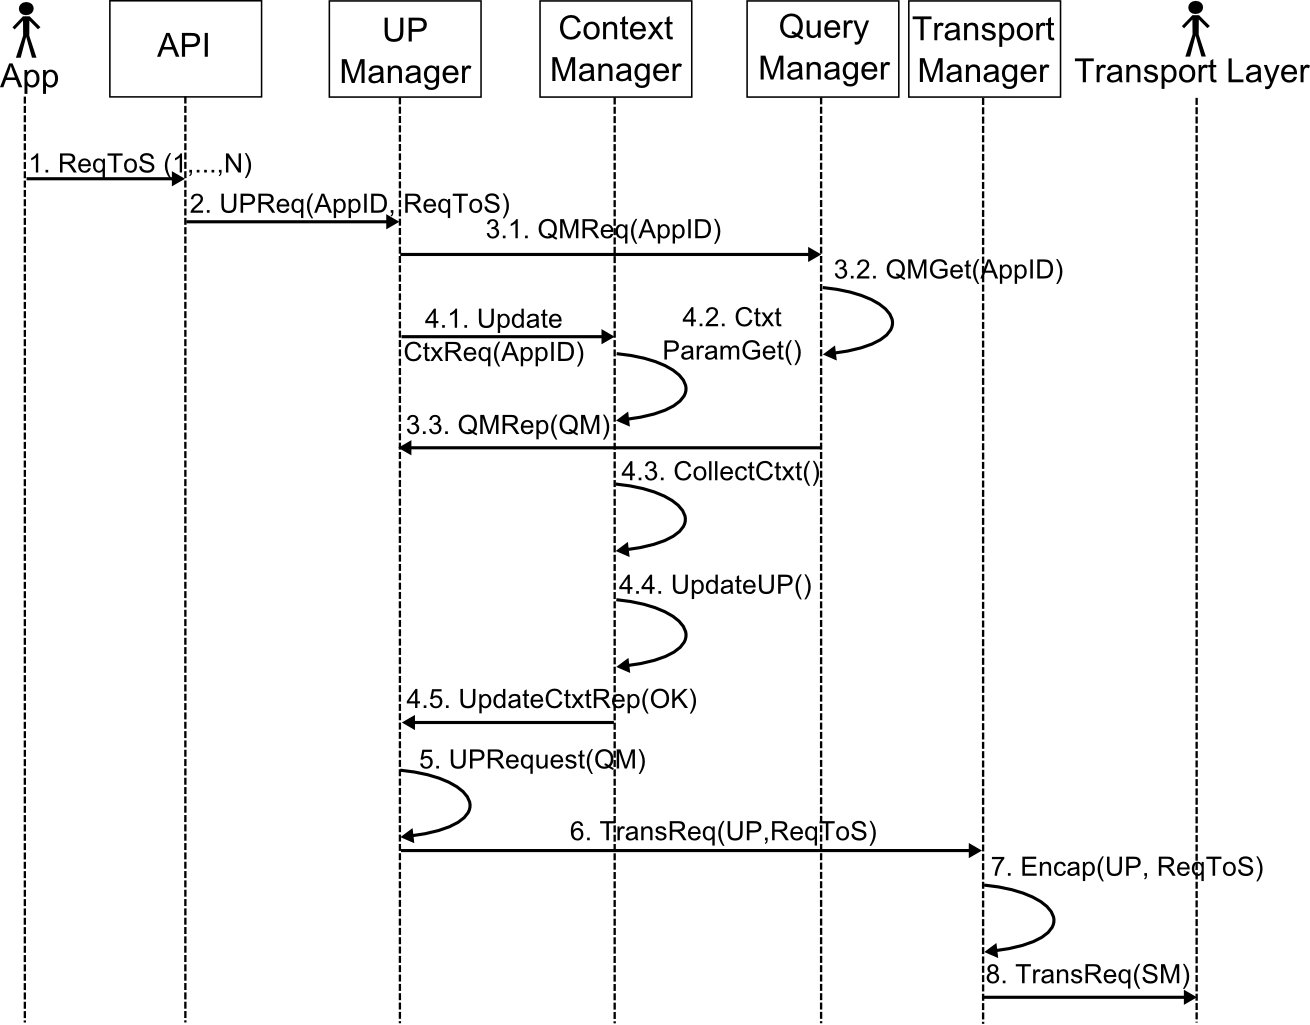
\includegraphics[width=0.5\textwidth]{imagens/chellouche2.png}
  \caption{Construção de perfil\cite{chellouche10}}
  \label{fig:chellouche2}
\end{figure}

%%%%%%%%%%%%%%%%%%%%%%%%%%%%%%%%%%%%%%%%%%%%%%%%%%%%%%%%%%%%%%%%%%%%%%%%%%

\subsection{Outros}

\textbf{[Avaliação de outros trabalhos relacionados]}

%%%%%%%%%%%%%%%%%%%%%%%%%%%%%%%%%%%%%%%%%%%%%%%%%%%%%%%%%%%%%%%%%%%%%%%%%%

\subsection{Avaliação dos Ambientes Pesquisados}

A Tabela~\ref{tab:comparacao} exibe um comparativo dos trabalhos apresentados, onde os seguintes fatores são levados em consideração:

\begin{description}
  \item[Interoperabilidade]: o modelo apresenta interoperabilidade -- caso positivo, se a mesma é sintática ou semântica;
  \item[Perfis dinâmicos]: o modelo de perfil permite que os perfis sejam atualizados de acordo com eventos externos, sem a interferência do usuário;
  \item[Armazenamento]: define onde ficam armazenados os perfis do usuário;
  \item[Sensível a contexto]: o contexto do usuário é levado em consideração na formação do perfil;
  \item[Utiliza trilhas]: as trilhas do usuário são levadas em consideração na construção do perfil;
  \item[Domínio]: o perfil é voltado para um domínio específico, ou se o mesmo permite que vários domínios possam ser utilizados.
\end{description}

\begin{table*}\centering\footnotesize
  \begin{tabular*}{1\textwidth}{@{}lcccccc@{}}
    \toprule
                                         & Interope-  & Perfis    & Armaze- & Sensibilidade & Utiliza & \\
    Trabalho                             & rabilidade & dinâmicos & namento & a contexto    & trilhas & Domínio \\
    \midrule
    Chellouche et al \cite{chellouche10} & Sintática  & Sim       & Servidor& Sim           & Não     & Serviços multimídia \\
    \bottomrule
  \end{tabular*}
  \caption{Comparação entre os trabalhos apresentados}
  \label{tab:comparacao}
\end{table*}

O modelo apresentado por Chellouche et al\cite{chellouche10} apresenta um \emph{middleware} que pode ser usado por diferentes aplicativos como um servidor central de perfis. Ele é voltado para aplicações móveis e, embora atualize parte do perfil como forma de oferecer suporte a sensibilidade a contexto, não permite que os aplicativos criem novos campos nem definam as regras para atualização dos campos existentes.
